\documentclass[nonacm, language=english, language=greek]{acmart}

\usepackage{alphabeta}
\usepackage[utf8]{inputenc} % Required for inputting international characters
\usepackage[T1]{fontenc} % Use 8-bit encoding
\usepackage{subcaption}

\usepackage{tikz}
\usepackage{dirtytalk}
\usepackage{smartdiagram}
\usepackage{hyperref}
\usetikzlibrary{shapes.geometric, arrows}
\usetikzlibrary{timeline}

\tikzstyle{startstop} = [rectangle, rounded corners, minimum width=3cm, minimum height=1cm,text centered, draw=black, fill=red!30]
\tikzstyle{io} = [trapezium, trapezium left angle=70, trapezium right angle=110, minimum width=3cm, minimum height=1cm, text centered, draw=black, fill=blue!30]
\tikzstyle{process} = [rectangle, minimum width=3cm, minimum height=1cm, text centered, draw=black, fill=orange!30]
\tikzstyle{decision} = [diamond, minimum width=3cm, minimum height=1cm, text centered, draw=black, fill=green!30]
\tikzstyle{arrow} = [thick,->,>=stealth]


\newcommand{\en}[1]{\textlatin{#1}}
\newcommand{\src}[1]{\texttt{\en{#1}}}

%%
%% \BibTeX command to typeset BibTeX logo in the docs
\AtBeginDocument{%
  \providecommand\BibTeX{{%
    Bib\TeX}}}

%% Rights management information.  This information is sent to you
%% when you complete the rights form.  These commands have SAMPLE
%% values in them; it is your responsibility as an author to replace
%% the commands and values with those provided to you when you
%% complete the rights form.
\setcopyright{acmcopyright}
\copyrightyear{2022}
\acmYear{2022}
\acmDOI{}



%% If you are preparing content for an event
%% sponsored by ACM SIGGRAPH, you must use the "author year" style of
%% citations and references.
\bibliographystyle{ACM-Reference-Format}

%%
%% end of the preamble, start of the body of the document source.
\begin{document}

%%
%% The "title" command has an optional parameter,
%% allowing the author to define a "short title" to be used in page headers.
\title{Σχεδιασμός και Υλοποίηση Ιστοσελίδας Υποστήριξης Κοινότητας}

%%
%% The "author" command and its associated commands are used to define
%% the authors and their affiliations.
%% Of note is the shared affiliation of the first two authors, and the
%% "authornote" and "authornotemark" commands
%% used to denote shared contribution to the research.
\author{Ευάγγελοσ Λάμπρου}
\email{e.lamprou@upnet.gr}
\orcid{}
\affiliation{%
  \institution{Πανεπιστήμιο Πατρών}
  \streetaddress{}
  \city{}
  \state{}
  \country{}
  \postcode{}
}

\author{Απόστολοσ Παπαδημητρίου}
\affiliation{%
  \institution{Πανεπιστήμιο Πατρών}
  \streetaddress{}
  \city{}
  \country{}}
\email{a.papadimitriou@upnet.gr}

%% The abstract is a short summary of the work to be presented in the
%% article.
\begin{abstract}
    Στα πλαίσια αυτής της εργασίας γίνεται ο σχεδιασμός και η υλοποίηση μίας 
    ιστοσελίδας Υποστήριξης Κοινότητας. Γίνεται ανάλυση των απαραίτητων 
    λειτουργιών για την εφαρμογή και περιγράφεται το σύνολο των τεχνολογιών 
    που χρησιμοποιήθηκαν με εστίαση σε αξιοσημείωτα μέρη της υλοποίησης.
\end{abstract}

\maketitle

\section{Εισαγωγή}

Το θέμα της εφαρμογής που επιλέξαμε να σχεδιάσουμε στα πλαίσια του μαθήματος είναι Εφαρμογή Υποστήριξης Κοινότητας (\en{Productivity Website}). Ο λόγος που διαλέξαμε αυτό το θέμα είναι ότι θέλαμε να δημιουργήσουμε μία εφαρμογή που θα βοηθούσε τους χρήστες να ασχολούνται περισσότερο με τις ασχολίες τους.
Έχοντας πολλές φορές αμελήσει μία ασχολία που θέλαμε να κάνουμε, σκεφτηκαμε οτι κύριοι λόγοι που συμβαίνει είναι:
\begin{itemize}
    \item Έλλειψη χρόνου
    \item Ελάχιστες γνώσεις επί του θέματος
    \item Ελλειψη βοηθειας
    \item Χάσιμο ενδιαφέροντος
\end{itemize}

Έχοντας λοιπόν αναγνωρίσει μερικούς παράγωντες , παρατηρήσαμε ότι μπορούμε να δημιουργήσουμε μία εφαρμογή που θα μπορούσε να βοηθήσει τους χρήστες τις να ασχολούνται με τα \en{Hobbies} τους περισσότερο.
Ο τρόπος που θα το κάνει η εφαρμογή μας είναι με την διασύνδεση χρηστών με παρόμοιες ασχολίες.
Έτσι κάθε χρήστης μπορεί να βοηθάει ο ένας τον άλλο καθώς:
\begin{itemize}
    \item Θα μοιράζονται γνώσεις
    \item Θα μοιράζονται απόψεις
    \item Θα παρακινεί ο ένας τον άλλο
\end{itemize}

\section{Εννοιολογικόσ Σχεδιασμόσ}

\subsection{Λειτουργικές Απαιτήσεις}

Έχοντας διαλέξει τον στόχο της εργασίας μας, βρήκαμε και συγκρίναμε άλλες εφαρμογές τύπου \en{Forum} και καταγράψαμε τις λειτουργίες τους.
Κρατήσαμε τις λειτουργίες που θεωρήσαμε πιο χρήσιμες και προσθέσαμε τις λειτουργίες που χρειαζόμασταν προκειμένου η εφαρμογή μας να ανταποκρίνεται στις απαιτήσεις μας.

\subsubsection{Βασικές λειτουργίες}

\paragraph{Κεντρική Σελίδα} 
Η κεντρική σελίδα που βλέπει κάθε επισκέπτης της εφαρμογής. Περιέχει διάφορες
ενδιαφέρουσες πληροφορίες για την εφαρμογή (Κορυφαίες δραστηριότητες, χρήστες
κτλπ), ώστε να δώσει στον επισκέπτη κάτι νεο για να επισκεφτεί.
 
\paragraph{Προφίλ Χρήστη}
Μία σελίδα που έχει πληροφορίες για τον αντιστοιχο χρήστη. Στην δικιά μας περίπτωση την εικόνα προφιλ, λίγα λόγια απο τον χρήστη, τις δραστηριότητες που συμμετέχει κτλπ.
 
\paragraph{Δημιουργία και σύνδεση νέου Χρήστη}
Την δυνατότητα κάποιος επισκέπτης της εφαρμογής να δημιουργήσει νέο λογαριασμό ή να συνδεθεί σε ένα ήδη υπάρχων. Έτσι ώστε να μπορεί να συμμετέχει σε δραστηριότητες και να διασυνδεθεί με άλλους χρήστες με παρόμοιες ασχολίες.
 
\paragraph{\en{Session} (Συνεδρία) Χρήστη} 
Την δυνατότητα να κρατάμε την πληροφορία για όταν συνδέεται ένας χρήστης, ώστε να αλλάζουν οι λειτουργίες της εφαρμογής.
 
\paragraph{Σελίδα δραστηριοτήτων}
Μία σελίδα που παρουσιάζει εν συντομία τις δραστηριότητες που υπάρχουν στην εφαρμογή, καθώς και τον αριθμό χρηστών και αναρτήσεων που έχουν γίνει σε αυτές.
 
\paragraph{Εγγραφή και απεγγραφή σε δραστηριότητες}
Την δυνατότητα ένας συνδεδεμένος χρήστης να εγγράφεται και να απεγγράφεται από μία δραστηριότητα.
 
\paragraph{Δημιουργία αναρτήσεων}
Την δυνατότητα οι συνδεδεμένοι χρήστες να δημιουργούν νέες αναρτήσεις για μια δραστηριότητα, ώστε να μοιράζονται απόψεις, ερωτήσεις και προσωπικά επιτεύγματα.
 
\paragraph{Σχολιασμός αναρτησεων}
Την δυνατότητα οι συνδεδεμένοι χρήστες να σχολιάζουν αναρτήσεις, ώστε να μπορούν να συζητούν και να μοιράζονται γνώσεις και εμπειρίες.
 
\subsubsection{Μη βασικές λειτουργίες}

\paragraph{Δημιουργία φίλων}
Την δυνατότητα να προσθέτει ένας χρήστης έναν άλλο, με σκοπό να μπορεί να
ενημερώνεται γρήγορα για τις δραστηριότητες που συμμετέχει και τις ενέργειες
του σε αυτές. Κάτι που αξίζει να σημειωθεί, είναι ότι δεν θέλαμε να
δημιουργηθεί το γνωστό κοινωνικό πρόβλημα με τους "ακόλουθους", που
εμφανίζεται(υπάρχει?) σε άλλες εφαρμογές κοινωνικής δικτύωσης. Προκειμένου να
αποτρέψουμε τους χρήστες μας από το να τους γίνεται έμμονη ιδέα(ή να
επικεντρώνονται?) τα νούμερα αλλων χρηστών που τους ακολουθούν, αποφασίσαμε να
μην εμφανίζεται πουθενά αυτό το στατιστικό. Έτσι θέλαμε να προωθήσουμε (ή
καλλιεργήσουμε) ένα κλίμα αλληλοβοήθειας, μιας και ο λόγος που υπάρχουν οι
φίλοι στην εφαρμογή ,είναι να ενημερώνονται γρήγορα οι χρήστες για την
δραστηριότητα των φίλων τους στην κοινότητα.

\paragraph{Άντληση ενδιαφερόντων στατιστικών}
Την δυνατότητα να αντλούνται ενδιαφέροντα στατιστικά για τις δραστηριότητες και
τους χρήστες. Όπως πόσες αναρτησεις δημιουργούνται ανά μήνα, πόσα σχόλια
δημιουργούνται ανά μήνα κτλπ.

\paragraph{Μοναδικές εικόνες προφίλ}
Την δυνατότητα κάθε χρήστης να έχει μία μοναδική εικόνα προφίλ. Η εικόνα προφίλ
δημιουργείται αυτόματα με βάση το όνομα του χρήστη και είναι μοναδική. Έτσι
κάθε χρήστης μπορεί να έχει μια μοναδική εικόνα αυτόματα χωρίς να πρέπει να
κάνει κάτι.

\paragraph{Απάντηση σε σχόλια}
Την δυνατότητα ένας χρήστης να απαντάει άμεσα σε ένα σχόλιο, προκειμένου να μπορούν να δημιουργούνται συζητήσεις. Επίσης δόθηκε αρκετή σημασία στο να εμφανίζονται σωστά οι απαντήσεις στα σχόλια, προκειμένου να είναι πιο εύκολη η ανάγνωση μίας συζήτησης και η συμμετοχή σε αυτή.

\paragraph{Εμφανιση κειμενου σε \en{Markdown}} 
Την δυνατότητα να γράφεται κείμενο στην γλώσσα \en{Markdown}, έτσι ώστε οι χρήστες να μπορούν να γράφουν εμπλουτισμένο κείμενο το οποίο θα εμφανίζεται σωστά.

\paragraph{Λειτουργίες διαχειριστων κοινοτητας (Εισαγωγή νέων δραστηριοτήτων, Διαγραφή σχολίων κτλπ.)}
Την δυνατότητα να μπορούν διαχειριστές να συντηρούν και να φροντίζουν τις
κοινότητες που υπάρχουν στην εφαρμογή, καθώς και να προσθέτουν καινούργιες
δραστηριότητες. (Ίσως να αναφερθει αργοτερα οτι θα θελαμε να το βελτιώσουμε;)

\subsection{Βάση Δεδομένων}

Ο σχεδιασμός της βάσης δεδομένων έγινε με δύο βασικούς στόχους. 

\begin{itemize}
    \item Την αποτύπωση όλων των βασικών λειτουργιών της ιστοσελίδας.
    \item Την απλότητα της υλοποίησης.
\end{itemize}

Το τελικό σχεδιάγραμμα δεν έχει ιδιαιτερότητας. Τα μόνα 
αξιοσημείωτα κομμάτια του είναι οι αναδρομικές σχέσεις 
της φιλίας και της απάντησης σε σχόλιο οι οποίες προκύπτουν 
από την συμμετρική φύση αυτών των πράξεων.

\begin{figure}[htpb]
    \centering
    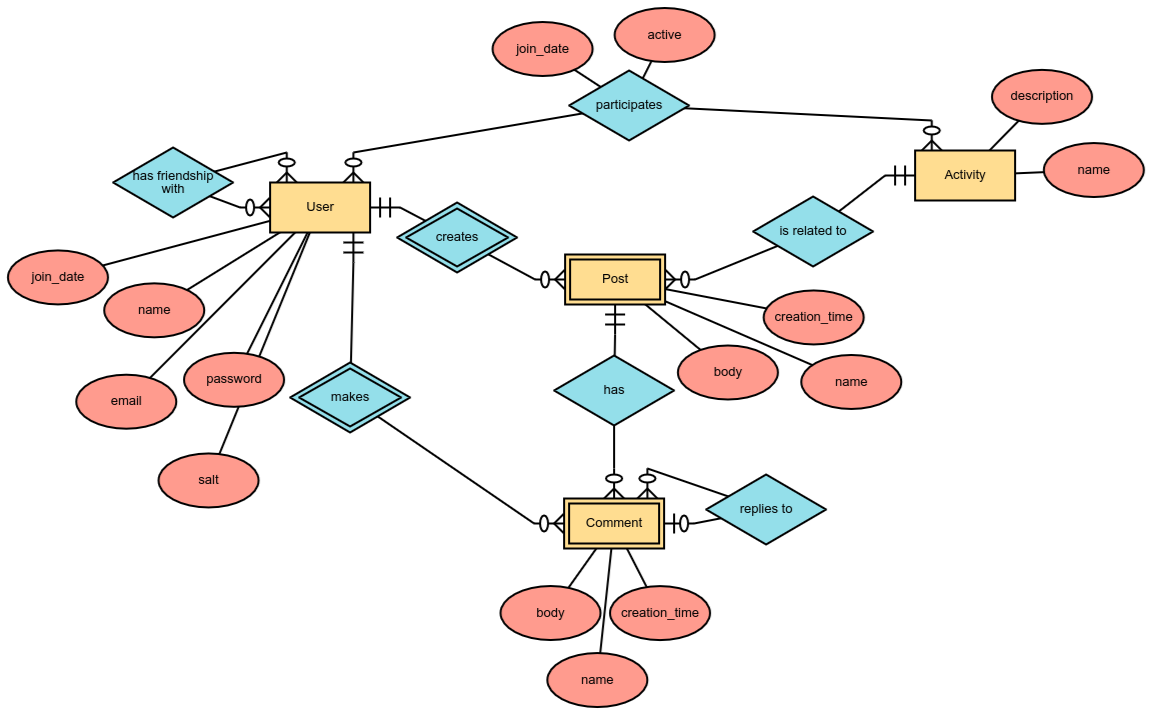
\includegraphics[width=\textwidth]{./assets/erd.png}
    \caption{Το διάγραμμα οντοτήτων-συσχετίσεων για την εφαρμογή μας.}
    \label{fig:}
\end{figure}

\subsection{Διάγραμμα Ροής Χρήστη}

Το διάγραμμα ροής χρήστη αποτυπώνει τις σελίδες στις οποίες μπορεί να έχει 
πρόσβαση ο χρήστης. Με βάση την τωρινή του κατάσταση έχει πρόσβαση σε 
διαφορετικά μέρη της ιστοσελίδας.

\begin{figure}[H]
\begin{center}
\begin{tikzpicture}[node distance=3.5cm, scale=0.6, every/.style={transform shape}]

    \node (start) [startstop] {Αρχική Σελίδα};

    \node (loggedin)        [decision, below of=start]         {\footnotesize Συνδεδεμένος?};
    \node (activitiespage)  [process, left of=loggedin]        {Δραστηριότητες};
    \node (postspage)       [process, below of=activitiespage] {Αναρτήσεις};
    \node (postpage)        [process, below of=postspage]      {Ανάρτηση};
    \node (profile)         [process, below of=postpage]       {Προφίλ Χρήστη};
    \node (loginpage)       [process, below of=loggedin]       {Σύνδεση};
    \node (registered)      [decision, below of=loginpage]     {\footnotesize Εγγεγραμένος?};
    \node (loginsucess)     [decision, below of=registered]    {\footnotesize Επιτυχια?};
    \node (registerpage)    [process, right of=registered]     {Εγγαρφή};
    \node (personalprofile) [process, right of=loggedin]       {Προσωπικό προφίλ};

    \draw [arrow] (start)          -- (loggedin);
    \draw [arrow] (start)          -| (activitiespage);
    \draw [arrow] (loggedin)       -- node[right] {όχι} (loginpage);
    \draw [arrow] (loggedin)       -- node[above] {ναι} (personalprofile);
    \draw [arrow] (loginpage)      -- (registered);
    \draw [arrow] (registered)     -- node[above] {όχι} (registerpage);
    \draw [arrow] (registered)     -- node[right] {ναι} (loginsucess);
    \draw [arrow] (loginsucess)    -- node[right] {ναι} (personalprofile);
    \draw [arrow] (registerpage)   |- (loginpage);
    \draw [arrow] (activitiespage) -- (postspage);
    \draw [arrow] (postspage)      -- (postpage);
    \draw [arrow] (postpage)       -- (profile);
    \draw [arrow] (start)       -- (postspage);
    \draw [arrow] (start)       -- (profile);

\end{tikzpicture}
\end{center}
    \caption{Το διάγραμμα ροής χρήστη της εφαρμογής.}
    \label{fig:userflowdiagram}%
\end{figure}
\section{Υλοποίηση}

\subsection{Τεχνολογίες}

Για την εργασία χρησιμοποιήσαμε τεχνολογίες οι οποίες 
είναι ήδη ευρέως διαδεδομένες στον χώρο του προγραμματισμού 
διαδικτύου. Οι περισσότερες από αυτές είχαν ήδη προταθεί 
στα πλαίσια του μαθήματος.
Για σύνθετες και συμπληρωματικές λειτουργικότητες έγινε 
χρήση εξωτερικών βιβλιοθηκών οι οποίες 
είτε βρίσκονται στην μεριά του \en{server} ως 
πακέτα ή τοποθετούνται εντός των \src{HTML} σελίδων 
οι οποίες σερβίρονται ως \en{inline-scripts} που πρσφέρονται 
μέσω \src{CDN}. \cite{CDN} Για κάθε μία από αυτές γίνεται ειδική αναφορά.

\subsubsection{Τεχνολογίες \en{Front-End}}

Για το \en{front-end} μέρος της εφαρμογής ως βάση έχουμε τις τεχνολογίες
\src{HTML} και \src{CSS} με τις οποίες χειριζόμαστε την δομή και το στυλ της
σελίδας αντίστοιχα. Ακόμα, υπάρχουν ορισμένα σημεία στα οποία με
\src{Javascript} από την πλευρά του χρήστη γίνεται η υλοποίηση δυναμικών
στοιχείων της σελίδας. 

Βασικός στόχος της εργασίας ήταν η υλοποίηση \en{responsive} σελίδων, οι οποίες
να παρουσιάζουν το περιεχόμενό τους εύλογα ανεξαρτήτως του μεγέθου της οθόνης
του χρήστη. Η βιβλιοθήκη \src{Bootstrap} \cite{Bootstrap} αποτελεί ένα σύνολο
από επαναχρησιμοποιούμενα κομμάτια κώδικα \src{CSS, HTML, Javascript}. Ο
βασικός τρόπος με τον οποίο την χρησιμοποιήσαμε στην εργασία ήταν στη χρήση των
\src{CSS} κλάσεων για εύκολη διαχείριση της δυναμικότητας των αντικειμένων του
\src{DOM}, όπως και στην προσθήκη απλών διαδραστικών στοιχείων \en{(drop-down
lists)}.

Στις σελίδες των χρηστών, γίνεται χρήση της βιβλιοθήκης \src{Chart.js}
\cite{ChartJS}, η οποία προσφέρει εύκολη προσθήκη διδραστικών γραφημάτων.
Χρησιμοποιήθηκε για την παρουσίαση στατιστικών στοιχείων. Από την μεριά του
χρήστη δίνεται η δυνατότητα χρήσης συντακτικού \src{markdown} \cite{Markdown}.
Αυτό σημαίνει πως το σώμα ενός σχολίου, ανάρτησης ή η περιγραφή ενός προφίλ
μπορεί να είναι γραμμένη σε \src{markdown} και στον τελικό χρήστη να φαίνεται
το αντίστοιχο \en{HTML}. Η μετατροπή του κειμένου αυτού σε \src{HTML} γίνεται
μέσω της βιβλιοθήκης \src{marked}. \cite{Marked}

\subsubsection{Τεχνολογίες \en{Back-End}}

Από τη μεριά του \en{server} χρησιμοποιήσαμε
το λογισμικό \src{Node.js} \cite{Node.js}, 
το οποίο μας πρσοφέρει ένα \en{Javascript Runtime Environment} μέσω 
του οποίου μπορούμε να χρησιμοποιήσουμε τη γλώσσα \src{Javascript} 
για να υλοποιήσουμε τον \en{webserver}.

Όσων αφορά την διαχείριση των κλήσεων από τους χρήστες, την δρομολόγηση 
και το σερβίρισμα αρχείων \src{HTML} διαλέξαμε τη δημοφιλή 
βιβλιοθήκη \src{Express.js} \cite{Express}, η οποία απλοποιεί 
τις παραπάνω λειτουργικότητες. Η \src{express} προσφέρει 
ένα πολύ ισχυρό \en{API} μέσω του οποίου μπορύμε να βάζουμε 
\say{\en{middlewares}} στην εφαρμογή μας. Αυτά μπορούμε να τα 
σκεφτούμε σαν κομμάτια κώδικα τα οποία έχουν σαν είσοδο μία αίτηση 
ή απάντηση από/προς τον εξυπηρετητή και ως έξοδο μία εμπλουτισμένη έκδοσή 
της. Πάνω σε αυτή την τεχνολογία πατάνε πολλές άλλες βιβλιοθήκες οι οποίες 
προσφέρουν περίπλοκες λειτουργικότητες, με τον προγραμματιστή ωστόσο 
να μπορεί να τις ενσωματώσει πολύ εύκολα στην εφαρμογή του.

Για το σερβίρισμα αρχείων \src{HTML}, με σκοπό να έχουμε 
πιο ευανάγνωστο κώδικα \src{HTML} και να αποφύγουμε τις δυσκολίες 
που συνδέονται με \en{client-side rendering}, χρησιμοποιήσαμε 
τη βιβλιοθήκη \src{Handlebars} \cite{Handlebars}. Εφόσων δεν 
χρησιμοποιήσαμε κάποιο \en{UI Framework}, το εργαλείο αυτό διευκόλυνε 
σε μεγάλο βαθμό την ανάπτυξη των πιο σύνθετων σελίδων της εφαρμογής.
Η \src{Handlebars} δίνει τη δυνατότητα ενσωμάτωσης λογικής 
όπως \en{ifs, for-loops} κλπ. ανάμεσα σε \src{HTML} κώδικα. 
Η τελική σελίδα παράγεται έτσι από τον \en{server} και παρουσιάζεται στον χρήστη.
Η τεχνική αυτή παραγωγής σελίδων αν και πλέον ξεπερασμένη, με την επικράτηση 
της παραγωγής στοιχείων της σελίδας δυναμικά από την πλευρά του \en{client}, μπορεί να κάνει 
πιο εύκολη την απασφαλμάτωση της εφαρμογής, εφόσων το τί έστειλε ο \en{server}
και τί βλέπει τελικά ο \en{browser} ταυτίζονται.

Η διαχείριση της σύνδεσης χρηστών γίνεται από τη βιβλιοθήκη \en{Passport}.
\cite{Passport} Αυτή λειτουργεί σαν μεσάζωντας μεταξύ μία αίτησης του χρήστη
για εγγραφή/σύνδεση και της βάσης δεδομένων. Τελικά, προστίθεται σε κάθε αίτηση
(\en{request}) πληροφορία για την ταυτότητα του χρήστη. Αυτή η λειτουργικότητα
γίνεται μέσω της βιβλιοθήκης \src{express-session}. 

Για την μόνιμη αποθήκευση των στοιχείων της εφαρμογής χρησιμοποιήσαμε τη
βάση δεδομένων \en{MySQL} και συγκεκριμένα την ανοιχτή υλοποίηση του
\en{MariaDB}. \cite{MariaDB}. Πληροφορίες για το κάθε \en{session} 
αποθηκεύονται σε βάση \en{SQLite}.

Η διαφοροποίηση μεταξύ της βάσης για τις πληροφορίες που αφορόυν την λειτουργικότητα της 
εφαρμογής και της βάσης αποθήκευσης πληροφοριών συνεδρίασης έγινε για χάρην ευκολίας, 
μιας και ο χειρισμός μιας \en{SQLite} βάσης είναι αρκετά πιο απλός και υποστηρίζεται
άμεσα από τη βιβλιοθήκη \src{express-session}.

\begin{figure}[htpb]
    \centering
\smartdiagram[descriptive diagram]{
    {\en{Bootstrap}, {Έτοιμα \src{CSS/Javascript} \en{components}}},
    {\en{Handlebars}, {\src{HTML} \en{Render Engine}}},
    {\en{Express}, {\en{WebServer}}},
    {\en{Node}, {Περιβάλλον εκτέλεσης \src{Javascript}}},
    {\en{MySQL/SQLite}, {\en{DataBase Management System}}},
}
    \caption{Τα βάσικα μερή του \en{technology stack} που χρησιμοποιήσαμε.}
    \label{fig:}
\end{figure}



\subsection{Λειτουργικότητα Εφαρμογής}

\paragraph{Αρχική Σελίδα}

Η εμπειρία χρήσης ξεκινάει με την αρχική σελίδα. 
Εδώ παρουσιάζονται ορισμένες πληροφορίες σχετικά με
δημοφιλείς δραστηριότητες και κορυφαίους χρήστες. 
Ο υπολογισμός αυτών γίνεται με βάση τον αριθμό των πρόσφατων δημοσιοποιήσεων.

Ο χρήστης εφόσων δεν είναι συνδεδεμένος ακόμα μπορεί να: 

\begin{itemize}
    \item Βλέπει προφίλ άλλων χρηστών.
    \item Βλέπει δημοσιεύσεις των υπάρχοντων δραστηριοτήτων.
\end{itemize}

\paragraph{Σύνδεση}

Ο χρήστης μπορεί να συνδεθεί στη σελίδα \say{\en{Login}}. Σε περίπτωση που δεν
υπάρχει το όνομα στη βάση ή ο κώδικός είναι λανθασμένος ο χρήστης ενημερώνεται
με \en{pop-up}. Υπεύθυνη για την προσπάθεια σύνδεσης και την παραγωγή μυνημάτων
σφάλματος είναι η βιβλιοθήκη \src{passport.js}. 

\paragraph{Εγγραφή}

Αν δεν υπάρχει το όνομα του χρήστη ακόμα στη βάση μπορεί να φτιάξει λογαριασμό
στη σελίδα \say{\en{Register}}. Η εγγραφή του χρήστη στη βάση γίνεται επίσης
μέσω της βιβλιοθήκης \src{passport.js} \cite{Passport}.

Για την αποθήκευση των κωδικών φροντίσαμε να τους περάσουμε πρώτα από 
ένα \en{hash function} (\src{SHA-256} \cite{SHA256}), σε συνδυάσμο 
με ένα \en{string} από τυχαία \en{bytes}, το \en{salt}.
Στα πλαίσια της εργασίας, η ασφάλεια των δεδομένων των χρηστών δεν είναι 
σημαντικός παράγοντας, ωστόσο θέλαμε η ιστοσελίδα να είναι προστατευμένη 
από τις πιο σύνηθεις επιθέσεις.

Αφού συνδεθεί ο χρήστης, του αντιστοιχείται πλέον ένα \en{session-token}. Έτσι,
μπορούμε να αποθηκεύουμε πληροφορίες σχετικά με τη συνεδρία του. Στην εφαρμογή,
οι μόνες πληροφορίες που αξιοποιούμε για την παρουσίαση των σελίδων είναι το αν
ο χρήστης είναι συνδεδεμένος και το \en{id} που του αντιστοιχεί στη βάση
δεδομένων.

\paragraph{Προφίλ Χρήστη}

Μόλις συνδεθεί ο χρήστης, γίνεται ανακατεύθυνση του 
στη σελίδα με το προσωπικό του προφίλ. Εδώ του 
παρουσιάζονται πληροφορίες σχετικά με τις δραστηριότητες 
στις οποίες έχει συμμετάσχει. 
Δίνονται επίσης μερικές γραφικές παραστάσεις. Ο τρόπος με τον οποίο 
αυτές παράγονται είναι από την πλευρά του \en{client}, όπου γίνεται 
\en{request} στο \en{api} της ιστοσελίδας το οποίο επιστρέφει 
ένα \src{json} αντικείμενο με τα στατιστικά του χρήστη. 
Η βιβλιοθήκη \src{chart.js} \cite{ChartJS}
αναλαμβάνει την εμφάνιση των γραφημάτων.
Στο προφίλ του ο χρήστης μπορεί ακόμη να επεξεργαστεί την περιγραφή του 
(\en{bio}) και να δει τους χρήστες με τους οποίους είναι \say{φίλος}.

\paragraph{Σελίδες Δραστηριοτήτων/Δημοσιεύσεων}

Στη σελίδα \say{\en{Activities}}, γίνεται στην ουσία παρουσίαση του
περιεχομένου της βάσης, με τον χρήστη να μπορεί να δει τις δημοσιεύσεις και τα
σχόλια σε αυτές για κάθε διαφορετική δραστηριότητα. Ακόμα, ο χρήστης μπορεί να
δημιουργήσει νέες δημοσιεύσεις και σχόλια εφόσων έχει το δικαίωμα.

Φροντίσαμε σε ορισμένα \en{text-fields} να δίνεται η δυνατότητα 
στους χρήστες να εισάγουν κώδικα \src{markdown}. Στη συνέχεια 
θα θέλαμε να προσθέσουμε και τη δυνατότητα εισαγωγής \LaTeX κώδικα.

Μία από τις δυσκολίες στην σχεδίαση ήταν ο μηχανισμός απάντησης
σε κάποιο άλλο σχόλιο. Θέλαμε στη διεπαφή να φαίνεται 
ξεκάθαρα το ποιος χρήστης απαντάει σε ποιο σχόλιο
ώστε να δημιουργόυνται \say{νήματα} από σχόλια.
Αυτό γίνεται τοποθετώντας τα σχόλια μέσα σε διαδοχικά \src{divs}
τα οποία έχουν ιδιότητα \src{margin}. Έτσι, τα συνολικά 
\src{margins} προσθέτονται και έχουμε το σχόλιο να εμφανίζεται πιο μέσα 
όσο είναι μεταγενέστερα στο \en{thread}. Η υλοποίηση αυτής 
της λειτουργίας απαιτεί και την χρήση \en{javascript}, πέρα 
του \en{pre-processor} της \en{Handlebars}.

\section{Χρονοδιάγραμμα}

Ο χρόνος μας οργανώθηκε από την αρχή του εξαμήνου. Η αρχή της συνεργασίας έγινε
με σύγχρονες συναντήσεις. Ωστόσο, εφόσων είχαν παρθεί οι βασικές σχεδιαστικές
αποφάσεις και η εργασία είχε αρχίσει να παίρνει μορφή μπορούσαμε να δουλεύουμε
ασύγχρονα εκμεταλευόμενοι τα άριστα εργαλεία του \en{version control system}
\src{git} \cite{git} το οποίο χρησιμοποιήσαμε μέσα από την υπηρεσία
\en{GitHub}.

Σημεία της εφαρμογής στα οποία ένα μέλος της ομάδας ασχολήθηκε
αποκλειστικά είναι: 

\paragraph{Λάμπρου Ευάγγελος}
\begin{itemize}
    \item Λειτουργία \en{Login/Sessions}
    \item Εισαγωγή \en{markdown} σε φόρμες
    \item Δυναμική δημιουργία εικόνας προφίλ
\end{itemize}

\paragraph{Απόστολος Παπαδημητρίου}
\begin{itemize}
    \item Κατάλληλη παρουσίαση σελίδας σε συνδεδεμένους/μη χρήστες
    \item Λειτουργία πρσθήκης δημοσιεύσεων
    \item Λειτουργία προσθήκης σχολίων και 
        λειτουργία απάντησης σε σχόλιο
\end{itemize}

\begin{figure*}[!htb]
\begin{center}
    \begin{tikzpicture}[timespan=Ebdom`ada, timeline width=15, end week=10]
    
  \timeline{7}

  \begin{phases}
    \phase{between week=1 and 2 in 0.4,
      involvement degree=2.5cm,phase color=red!40!black}
    \phase{between week=3 and 5 in 0.5,
      involvement degree=3.5cm,phase color=red!90!black}
    \phase{between week=5 and 6 in 0.3,
      involvement degree=4cm,phase color=red!40!yellow}
    \phase{between week=6 and 7 in 0.3,
      involvement degree=5cm,phase color=red!40!blue}
  \end{phases}

  \addmilestone{at=phase-1.120,direction=90:1cm, text={Επιλογή Θέματος}, text options={above}}
  \addmilestone{at=phase-1.270,direction=270:1cm, text={Αναζήτηση Παρόμοιων Εφαρμογών}, text options={below}}

  \addmilestone{at=phase-2.70, direction=90:1cm, text={Επιλογή Τεχνολογιών}, text options={above}}
  \addmilestone{at=phase-2.150, direction=90:1.0cm, text={Σχεδιασμός \en{Front-End}}, text options={above}}
  \addmilestone{at=phase-2.250, direction=270:2cm, text={Σχεδιασμός Βάσης}, text options={below}}

  \addmilestone{at=phase-3.90,direction=90:1.2cm, text={Δημιουργία Πρώτων Σελίδων}, text options=above}
  \addmilestone{at=phase-3.250,direction=270:0.8cm, text options=below, text={\en{Node App}}}
  \addmilestone{at=phase-3.270,direction=270:2cm, text={Εισαγωγή Βάσης}}

  \addmilestone{at=phase-4.50,direction=90:1.2cm, text={\en{Login,Sessions}}, text options=above}
  \addmilestone{at=phase-4.250,direction=270:3cm, text options=below, text={Βελτίωση της διεπαφής}}
  \addmilestone{at=phase-4.300,direction=270:5cm, text={Διεπαφή Βάσης, Τελικές Λειτουργίες}}

\end{tikzpicture}

\end{center}
    \caption{Το χρονοδιάγραμμα συνεργασίας.}
\end{figure*}

\bibliography{acmart}

\appendix

\section{Εγκατάσταση}

Ο προτεινόμενος τρόπος χρήσης της εφαρμογής είναι μέσω 
του \en{docker-image} που προσφέρουμε στο αποθετήριο. 
Αυτό θα ετοιμάσει ένα περιβάλλον εκτέλεσης της εφαρμογής 
σε συνδυασμό με μία λειτουργική βάση \en{MySQL}. 

Εναλακτικά, μπορεί να γίνει χειροκίνητη εγκατάσταση της εφαρμογής 
χρησιμοποιώντας τα συμπεριλαμβανόμενα \src{makefiles}.

Αναλυτικές οδηγίες βρίσκονται στο αποθετήριο: \en{\url{https://github.com/vagos/webdevproject}}.

\section{Χρήση}

Για την χρήση της εφαρμογής μπορεί κάποιος να εκτλέσει 
τον \en{Node server} τοπικά στον υπολογιστή του ή 
να χρησιμοποιήσει κάποια υπηρεσία φιλοξενίας 
\en{web} εφαρμογών. Σαφώς, αν κάποιος έχει πρόσβαση
σε κάποιον υλικό \en{server}, μπορεί να 
βάλει την εφαρμογή να τρέξει εκεί.

Σε αυτό το σημείο παραθέτουμε μερικά στιγμιότυπα 
της εφαρμογής.

\begin{figure}[htpb]
    \foreach \image in {main_page.png, activities.png, post.png, single_activity.png}
    {
        \begin{subfigure}[b]{0.4\textwidth}
        \centering
            \includegraphics[width=\textwidth]{./assets/\image}
        \end{subfigure}
    }
    \caption{Μερικές από τις βασικές σελίδες της ιστοσελίδας.}
    \label{fig:}
\end{figure}

\begin{figure}[htpb]
    \foreach \image in {profile1.png, profile2.png, sign_in.png}
    {
        \begin{subfigure}[b]{0.4\textwidth}
            \includegraphics[width=\textwidth]{./assets/\image}
        \end{subfigure}
    }
    \caption{Μερικές από τις βασικές σελίδες της ιστοσελίδας.}
    \label{fig:}
\end{figure}


\end{document}
\endinput
